
\section{Analysis strategy}
\label{sec:analysis}

In section we describe our analysis strategy, and in particular
the classification of each individual event into
different categories according to the event topology.
%
First of all we discuss the settings and nomenclature that
we will use for jet clustering in this work.
%
Then we move to discuss how $b$-tagging is simulated,
following closely the ATLAS techniques.
%
Then we discuss the categorisation of events between different
topologies, and how we can prioritise among them.


\subsection{Jet reconstruction}

In our study we will use different types of jet definitions,
depending of the type of analysis that needs to be performed, optimized
for the various possible event topologies.
%
Therefore, we being by enumerating the choices that we make.
%
The starting point after the parton shower is the clustering
of all final state particles.
%
In this work all the jet reconstruction algorithms
are obtained from the {\tt FastJet} program~\cite{Cacciari:2011ma},
v3.1.0.
%
We adopt the following terminology for the different types of jets
that we will use in this work:

\begin{itemize}
\item {\it Small-$R$ jets}.

  These are jets  reconstructed with the
  anti-$k_T$ clustering algorithm~\cite{Cacciari:2008gp} with $R=0.4$ radius.
  %
  When reconstructing small-$R$ jets, we will keep only
  those jets with transverse momentum $p_T \ge 40$~GeV
  and pseudo-rapidity $|\eta|<2.5$ within the central
  acceptance of ATLAS and CMS, jets that fail to satisfy these
  conditions are discarded.
  %
    

\item {\it Large-$R$ jets}.

  These jets are also constructed with the
  anti-$k_T$ clustering algorithm, now using a $R=1.0$ radius.
  %
  In order to be accepted, these large-$R$ jets should
  satisfy  $p_T \ge 200$~GeV and lie in a pseudo-rapidity range by
  $|\eta|<2.0$.
  %
  If these conditions are not satisfied, the jet is discarded.
  %
  The more restrictive range  in pseudo-rapidity
  as compared to the small-$R$ jets,
  is motivated by mimicking the  experimental requirements
  in ATLAS and CMS
  related to the track-jet-based calibration.

  In addition to the basic $p_T$ and $\eta$
  acceptance requirements, large-$R$ jets should also
  satisfy the  BDRS mass-drop tagger~\cite{Butterworth:2008iy}
  conditions, in order
  to enhance the discrimination of the signal over the background
  events.
  %
  For the BDRS mass-drop tagger, we use the {\tt FastJet} default
  parameters of  $\mu = 0.67$ and $y_{\textrm{cut}}= 0.09$.
  %
  As required, before the mass-drop tagger is applied, the large-$R$ jet
  constituents are reclustered with the Cambridge/Aachen
  algorithm~\cite{Dokshitzer:1997in,Wobisch:1998wt}.


  
\item {\it Small-$R$ subjets}.

  Once we have reconstructed a suitable large-$R$ jet, important
  information can be obtained by looking at the kinematics of
  the small-$R$ subjets.
  %
  These subjets will be obtained by reclustering the constituents
  of the large-$R$ jet, always with the  anti-$k_T$ algorithm,
  but this time with a smaller radius parameter $R=0.3$.
  %
  As we will discuss below, these small-$R$ subjets are the key of
  the $b$-tagging in the boosted category.
  %
  Small-$R$ subjets are required to have $p_T > 50$~GeV and $|\eta|<2.5$,
  else they are discarded.

  \end{itemize}


\subsection{$b$-tagging}

Given the final state that needs to be reconstructed in our case, the
optimisation of the $b$-tagging capabilities of the
LHC experiments is an essential requirement to optimise
the prospects for the observation of Higgs pair production.
%
The $b$-tagging used in this feasibility study is inspired
in the current and projected ATLAS settings, and below
we also comment on the differences and similarities with the
corresponding CMS strategy~\cite{Khachatryan:2011wq,Chatrchyan:2012jua}.
%
For each type of jet defined above, a different
$b$-tagging strategy is used, as we discuss now.

\begin{itemize}

\item {\it Small-$R$ jets}.

  These are $b$-tagged as follows.
  %
  If a small-$R$ jet has at least one $b$-quark among their constituents,
  it will be tagged as a $b$-jet with probability $f_b$.
  %
  If no $b$-quarks are found among the constituents
  of this jet, it can be still be tagged as a $b$-jet with
  a mistag rate of $f_l$.
  %
  Note that the probability of tagging a jet is not modified
  if more than one $b$-quark is found among the jet constituents.

  We only attempt to $b$-tag the four (two) hardest small-$R$ jets
  in the resolved (intermediate) category.
  %
  We find that
  trying to $b$-tag all
  small-$R$ jets that satisfy the acceptance cuts worsens the performance
  due to combinatorics.

  \item {\it Large-$R$ jets}.

    Large-$R$ jets are $b$-tagged by ghost-associating anti-$k_T$ $R=0.3$
    subjets (defined as above) to the original large-$R$ jets.
    %
    In particular,
    a large-$R$ jet is considered  double-$b$-tagged if both
    the leading and subleading subjets (where the ordering
    is done in the subjet $p_T$) are both individually $b$-tagged.
    %
    Note that we only attempt to $b$-tag the two leading subjets:
    trying to $b$-tag all subjets above the $p_T$ cut degrades
    the signal significance due to the increase in combinatorics.

    Therefore, in this work we will exploit the capabilities of
    the LHC experiment of double-$b$-tagging inside large-$R$ jets.
    %
    Below we comment on the dependence of our results if single-$b$-tagging
    would be performed also for the large-$R$ jets, as done
    for the small-$R$ jets.

    Concerning the $b$-tagging probabilities and the
    light jet mistag probabilities, there are taken
    the same as for small-$R$ jets.
    %
    Therefore, a large-$R$ jet where the two leading
    subjets have at least one $b$-quark will be tagged
    with probability $f_b^2$, if only one of the two leading
    subjets has a $b$-quark then the tagging probability is
    $2f_bf_l$, and if none of the two have $b$-quarks
    as constituents, the mistag rate will be
    $f_l^2$.


\end{itemize}

Concerning the actual values of the $b$-tag probability $f_b$ and
the $b$-mistag probability of light jets $f_l$, in this work
we adopt as baseline the values $f_b=0.8$ and $f_l=0.01$.
%
In Sect.~\ref{sec:optimisation} we study the dependence of
our results against variations of $f_b$ and $f_l$ both
using more conservative and more aggressive values.
%
There we also study the dependence of the results
on other analysis settings related to the performance of
the experiments, for example by varying the momentum smearing.

\subsection{Event categorisation and cut flow}
\label{sec:categorisation}

After having introduced the types of jet reconstruction
that we will use, as well as the $b$-tagging strategy,
we need to discuss the analysis strategy, including
the event categorization and the cut flow.

The basic idea of this work is similar to that in Ref.~\cite{Gouzevitch:2013qca}:
rather than concentrating only a specific event topology, such as boosted
or resolved, we aim to consistently combine the information from
the three possible event topologies: boosted, intermediate and
resolved, which we define now.
%
An important difference as compared to~\cite{Gouzevitch:2013qca}
is that here each category is optimised separately, and then
a exclusive categorisation is defined starting from the topology
where the signal significance is the best.

Let us therefore define the three event categories that
we use in this work:
\begin{itemize}
\item {\it Boosted category}.

  A given event is assigned to the {\it boosted} category if it
  contains at least two large-$R$ jets, defined as above,
  and where  the two leading large-$R$ jets have been
  successfully double-$b$-tagged.
  %
 Therefore, each of these two large-$R$ double-$b$-tagged jets corresponds to the
 decay products of one Higgs boson candidate.

\item {\it Intermediate category}.

  An event is assigned to the {\it intermediate} category if
  at least one large $R$ double-$b$-tagged jet is present.
  %
  If more than one is found, then the leading large-$R$ jet
  is assigned to be the first Higgs candidate.
  %
  In addition, we require at least two small-$R$ jets,
  which must be separated with respect to the large-$R$
  jet by at least an angular separation of $\Delta R\ge 1.0$.
  %
  These small-$R$ jets must be $b$-tagged as well.

  
  Then, the second Higgs boson candidate is reconstructed
  by selecting the two $b$-tagged small-$R$ jets that minimize the difference
  between the invariant mass of the large-$R$ jet, $m_{lR_1}$,
  with the invariant mass of the sum of the two small-$R$ jets,
  $m_{sR_1+sR_2}$, that is, ${\rm min}\lp m_{lR} -
  m_{sR_1+sR_2}\rp$, where $lR_1$ indicates the leading large-$R$ jet
  and $sR_1$ and $sR_2$ indicate the small-$R$ jets.m

\item {\it Resolved category}.

  Finally, let us define the {\it resolved} category.
  %
  An event is assigned to this category
  if at least
  four $b$-tagged small-$R$ jets are present.
  %
  The two Higgs candidates are then reconstructed out of the
  leading four small-$R$ jets in the event
  by considering all possibilities of forming two pairs of jets
  with invariant masses $m_{sR_1+sR_2}$ and 
$m_{sR_3+sR_4}$, respectively, and choosing the configuration that minimizes their difference $|m_{sR_1+sR_2} - m_{sR_3+sR_4}|$. 
  %
  The requirement of restricting this selection to only the four
  leading small-$R$ jets arises from the need to reducing the
  combinatorics from the fakes.
\end{itemize}
Note that in principle these three categories are not exclusive:
a given even can be assigned to more than one category, for
example, satisfying both the requirements of the boosted and resolved
categories at the same time.



Once a pair of Higgs boson candidates has been identified,
then events from each category are required to satisfy the usual
Higgs mass window cut, defined by
the following condition
\be
\label{higgsmasswindow}
|m_{h,j} - 125| < 40~{\rm GeV} \, , j=1,2 \, ,
\ee
where $m_{h,j}$ is the invariant mass of the two Higgs candidates
reconstructed as explained above.
%
We note that this cut is substantially looser as the corresponding
cut used in the typical ATLAS and CMS $h\to b\bar{b}$
analyses~\cite{Aad:2012gxa,Chatrchyan:2013zna}: the motivation
for this is that the MVA will take care of the optimisation of these
and other cuts that are not explicitly performed.


In Table~\ref{sec:categorisation} we summarize the definitions of each
category.
%
We emphasize again that each category is not exclusive of the others,
and in general there can be a substantial overlap
between the different categories.
%
In particular, this overlap is a direct consequence that
the different categories are optimised separately, as opposed
to the approach of~\cite{Gouzevitch:2013qca}, where optimisation
was performed simultaneously in the combination of exclusive categories.


%%%%%%%%%%%%%%%%%%%%%%%%%%%%%%%%%%%
\begin{table}[h]
  \centering
  \small
  \begin{tabular}{c|c|c|c}
    \hline
    &  Boosted  &  Intermediate  &  Resolved  \\
    \hline
    \hline 
    Jet selection  &  $\ge 2$ large-$R$ jets  & 1 large-$R$ jet, $\ge 2$ small-$R$
    jets  &  $\ge$ 4 small-$R$ jets \\
    \hline
    Jet cuts  & $p_T \ge 200$ GeV   &  $p_T \ge 200$ GeV (large-$R$ jet)
    &  $p_T \ge 40$ GeV \\
    &  & $p_T \ge 40$ GeV (small-$R$ jets)   &    \\
    &   $|\eta|<2.0$  & $|\eta|<2.0$ (large-$R$ jet) & $|\eta|<2.5$ \\
    &        & $|\eta|<2.5$ (small-$R$ jet)  &  \\
    \hline
    $b$-tagging  & 2 double-$b$-tags  & 1 double-$b$-tag & 4 single-$b$-tags \\
    &  & and 2 single-$b$-tags  &  \\
       & $\ge 2$ small-$R$ subjets  & &  \\
    &  $p_T^{\rm sj}\ge 50$ GeV &   &  \\
    \hline
    \end{tabular}
  \caption{\small Definition of the three event categories used in this
    work, together with the corresponding basic kinematical cuts.
    %
    The categories are not exclusive, and each event can satisfy the
    requirements of more than one category at the same time.  
\label{sec:categorisationTable}
  }
\end{table}
%%%%%%%%%%%%%%%%%%%%%%%%%%%%%%%%%%%%%%

As we will show now, the selection requirement and the kinematic cuts
for each of the categories in Table~\ref{sec:categorisationTable} have
been optimised independently.
%
First of all we have performed a inclusive analysis, and optimised
$S/\sqrt{B}$ in each of the three categories separately, including
the MVA.
%
We find that, in terms of signal significance, the ordering of
the categories is
\begin{enumerate}
\item Boosted 
\item Intermediate
  \item Resolved
  \end{enumerate}
and therefore for the final analysis we turn to an exclusive approach:
if an event satisfies the boosted requirements, it is kept for
these category, else we check if it suits the intermediate
requirements, and failing also this, the event is attempted
in the resolved categories.
%
The resulting exclusive event samples are then separately processes
through the MVA, as discussed in the next section.
%
This allows us to combine the significance of the dominant topology
(boosted) with that of the sub-leading categories, intermediate
and resolved.

\subsection{Cut optimisation}

In this section we motivate the various
kinematical cuts for the various categories.
%
As mentioned before, the cuts in each category have been separately
optimised in an inclusive analysis: it is only once we have determined
which is the dominant category that the analysis is made exclusive.
%
In this work, the results for each category have been derived
from the inclusive analysis,
and we show the various kinematic distributions immediately
below the corresponding cut has been applied.

In this section we only show a representative subset of
all available kinematic distributions, the complete
set of comparison plots can be found in the following
webpage:
\begin{center}
\url{http://www2.physics.ox.ac.uk/HH4b}
  \end{center}
In this webpage we also show the distribution of all
kinematic variables, including jet substructure variables,
which we don't cut explicitly but that are provided as
input to the multivariate analysis.
%
Also, we show here results for the boosted and resolved categories,
a comparison which allows to understand the cuts used for the
intermediate category as well.

\subsubsection{Boosted category}


We begin with the boosted category, which is the one that leads
to a higher signal significance.
%
First of all,
in Fig.~\ref{fig:cutplots1} we show
the $p_T$ distribution of the
  leading large-$R$ jet in the boosted category, comparing
  the shapes of the distribution in signal and background events.
  %
  All distributions have been normalized to their total integral.
  %
  We see that the background distribution
  falls off rather steeply than the signal, therefore
  suggesting that the boosted region should be
  advantageous to suppress the background.


%%%%%%%%%%%%%%%%%%%%%%%%%%%%
\begin{figure}[t]
\begin{center}
  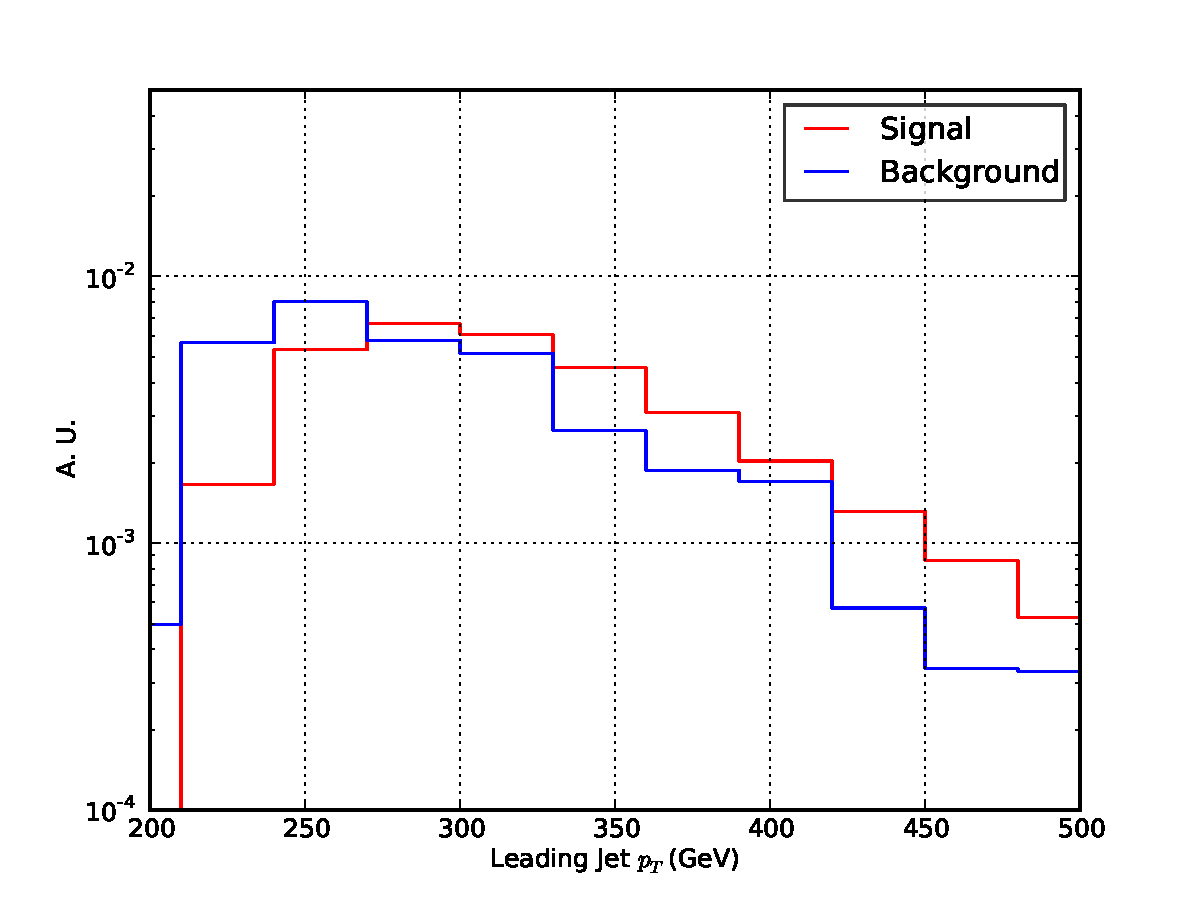
\includegraphics[width=0.48\textwidth]{plots/pt_H0_res_C1_boost.pdf}
  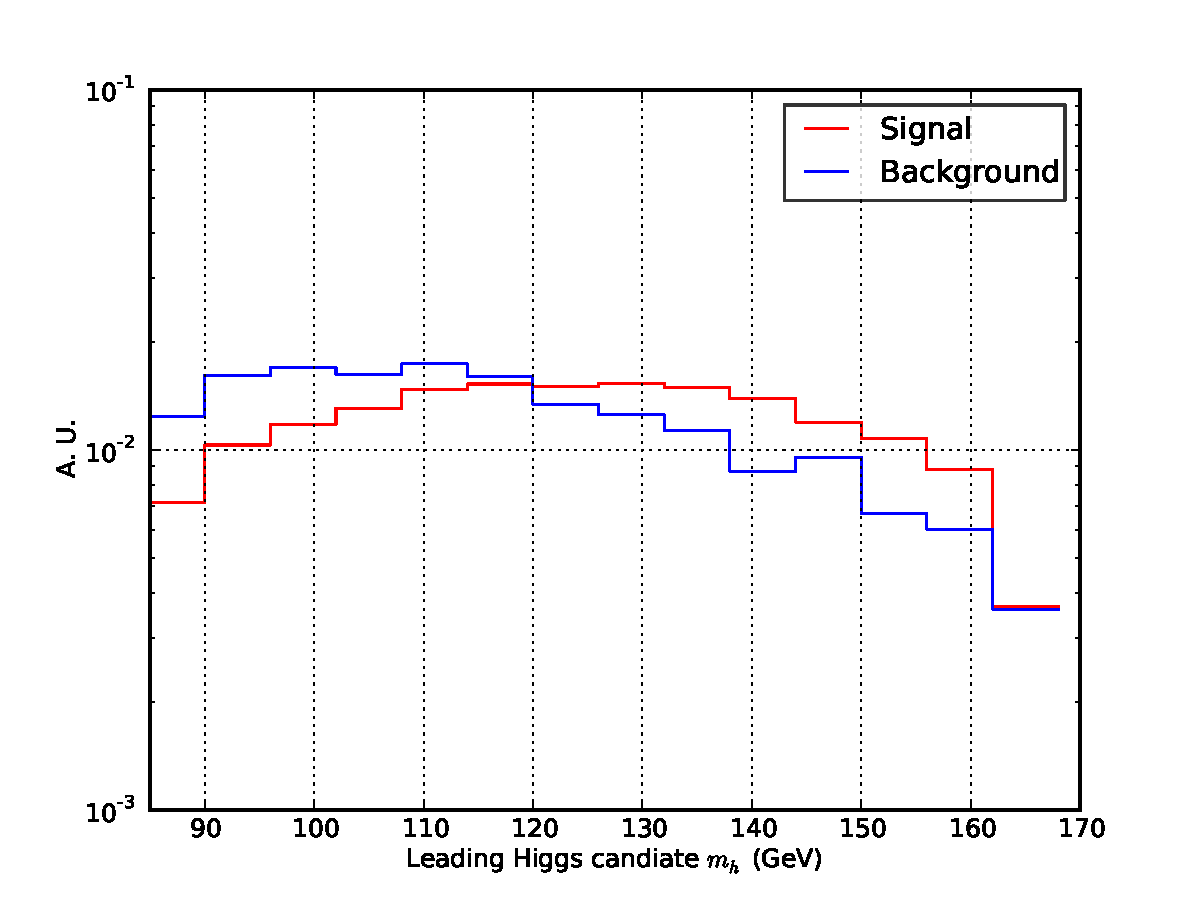
\includegraphics[width=0.48\textwidth]{plots/m_H0_res_C1_boost.pdf}
\caption{\small Left plot: the $p_T$ distribution of the
  leading large-$R$ jet in the boosted category, comparing
  the shapes of the distribution in signal and background events.
  %
  All distributions have been normalized to their total integral.
  %
  Right plot: the invariant mass of the leading Higgs
  candidate.
}
\label{fig:cutplots1}
\end{center}
\end{figure}
%%%%%%%%%%%%%%%%%%%%%%%

In Fig.~\ref{fig:cutplots1} we also show the distribution
of the invariant mass of the leading Higgs candidates.
%
The signal is of course well peaked at $m_h=125$ GeV, the physical
mass, while the background does not display any structure.
%
Note that the smearing, which mimics detector resolution effects,
leads to a rather broad distribution which reduces the usefulness
of the Higgs mass window cut.
%
However, the information of the different shape of the $m_{h}$
distribution will still be exploited by the MVA.

As explained above, in the boosted category we also require the two
leading subjets of the large-$R$ jet to be relatively
hard, in particular that should satisfy $p_T \ge $ 50 GeV.
%
To motivate this cut, in Fig ... we show the distribution in $p_T$ of the leading
and subleading sub-jets in the leading large-$R$ jet in events
of the boosted category.
%
It is clear from the comparison that the subjet $p_T$ spectrum is
relatively harder in the signal with respect to the background,
motivating our cut.

{\bf missing plots: pt subjet distribution}

\subsubsection{Resolved category}


Let's now consider the resolved category.
%
To begin with, here it is important to understand the $p_T$ distribution
of the four leading small-$R$ jets of the event.
%
Given that in general the boost from the Higgs decays is moderate,
the two subleading jets might be not too hard, and thus it
should be important to ensure that our $p_T^{\rm min}$ cut
is not too strong.
%
In Fig. we show the distribution in $p_T$ of the four leading
small-$R$ jets in signal and background events.
%
We see that the third and four leading jets are relatively soft.
%
Also, it is useful to show the distribution in rapidity of the
individual jets

{\bf missing plots: pt jet distribution, rapidity distribution}

Next, we show in
Fig.~\ref{fig:mhh} the invariant mass distribution of the Higgs pairs,
comparing the resolved category (left) with the boosted category (right)
%
This is interesting since it determines the degree of boost that the two
Higgs candidates will have after non-resonant production.
%
In the resolved case, we see that the distribution
in $m_{hh}$ is rather harder for the signal as for the background,
and thus one expects that cutting in $m_{hh}$ would help signal
discrimination: we will verify this with the MVA in the next section.
%
For the boosted category the trend of the $m_{hh}$ distribution
is very different because of the selection, with the
distribution now peaking at much higher values.
%
In this case signal and background distributions
look reasonably similar.



%%%%%%%%%%%%%%%%%%%%%%%%%%%%
\begin{figure}[t]
\begin{center}
  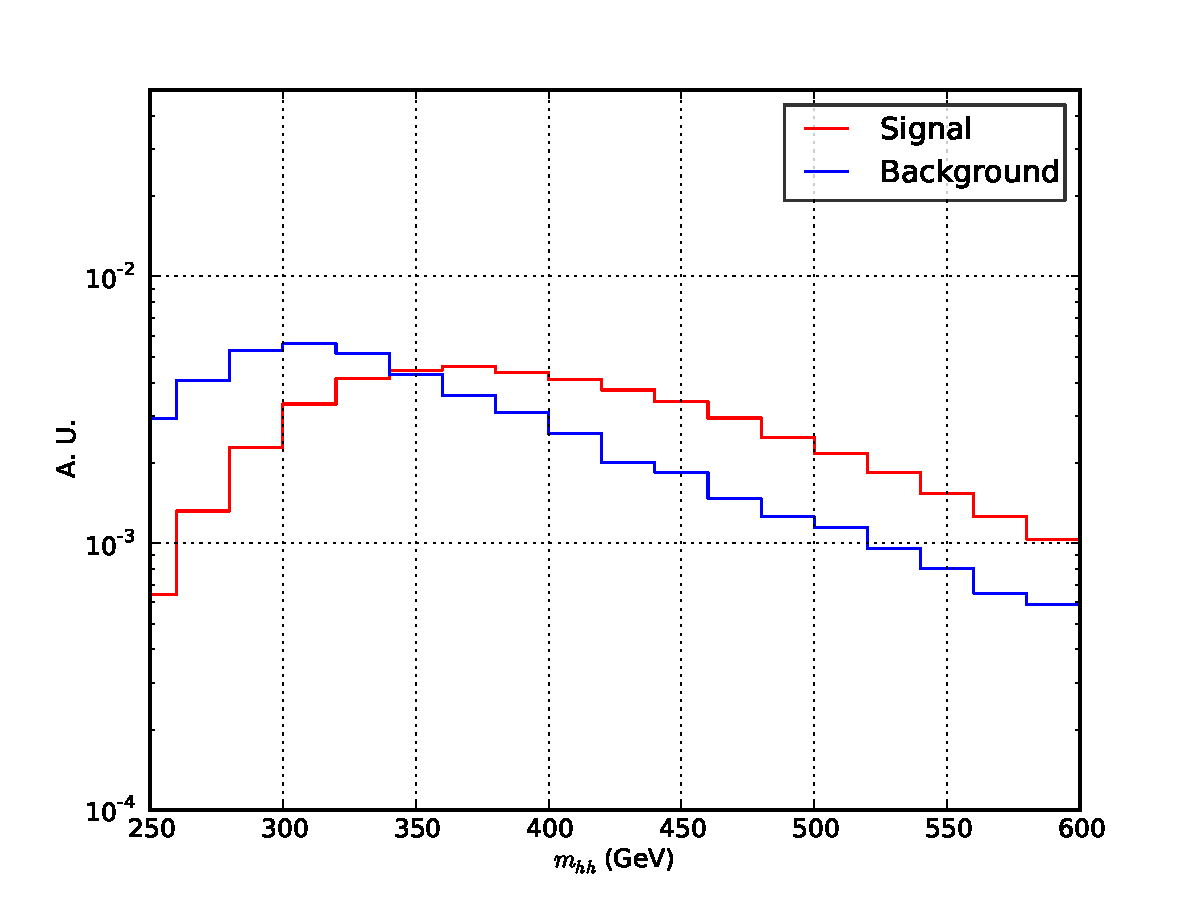
\includegraphics[width=0.48\textwidth]{plots/m_HH_res_C1.pdf}
  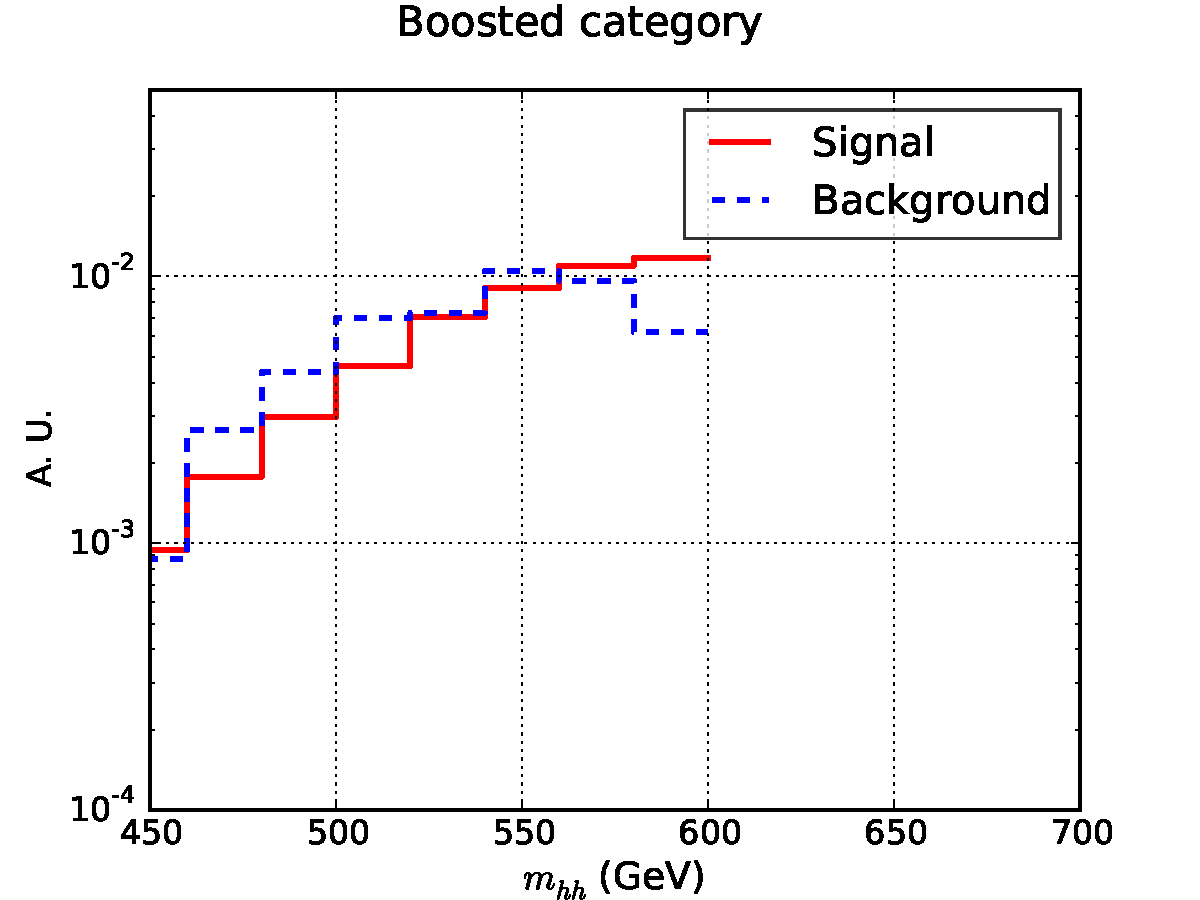
\includegraphics[width=0.48\textwidth]{plots/m_HH_boost_C1.pdf}
  \caption{\small Left plot: the invariant mass distribution of the Higgs
    pair candidates, $m_{hh}$, comparing signal and background events,
    in the resolved category.
    %
    Right plot: same for the boosted category.
}
\label{fig:mhh}
\end{center}
\end{figure}
%%%%%%%%%%%%%%%%%%%%%%%






